\section{DRL-Based QOCO Algorithm}
%\subsection{DQN-based solution}
%\subsection{Computation Model}

\begin{frame}
	\frametitle{DQN-based solution}
	
	\begin{figure}
	\captionsetup{name=Fig.}
	\centering
	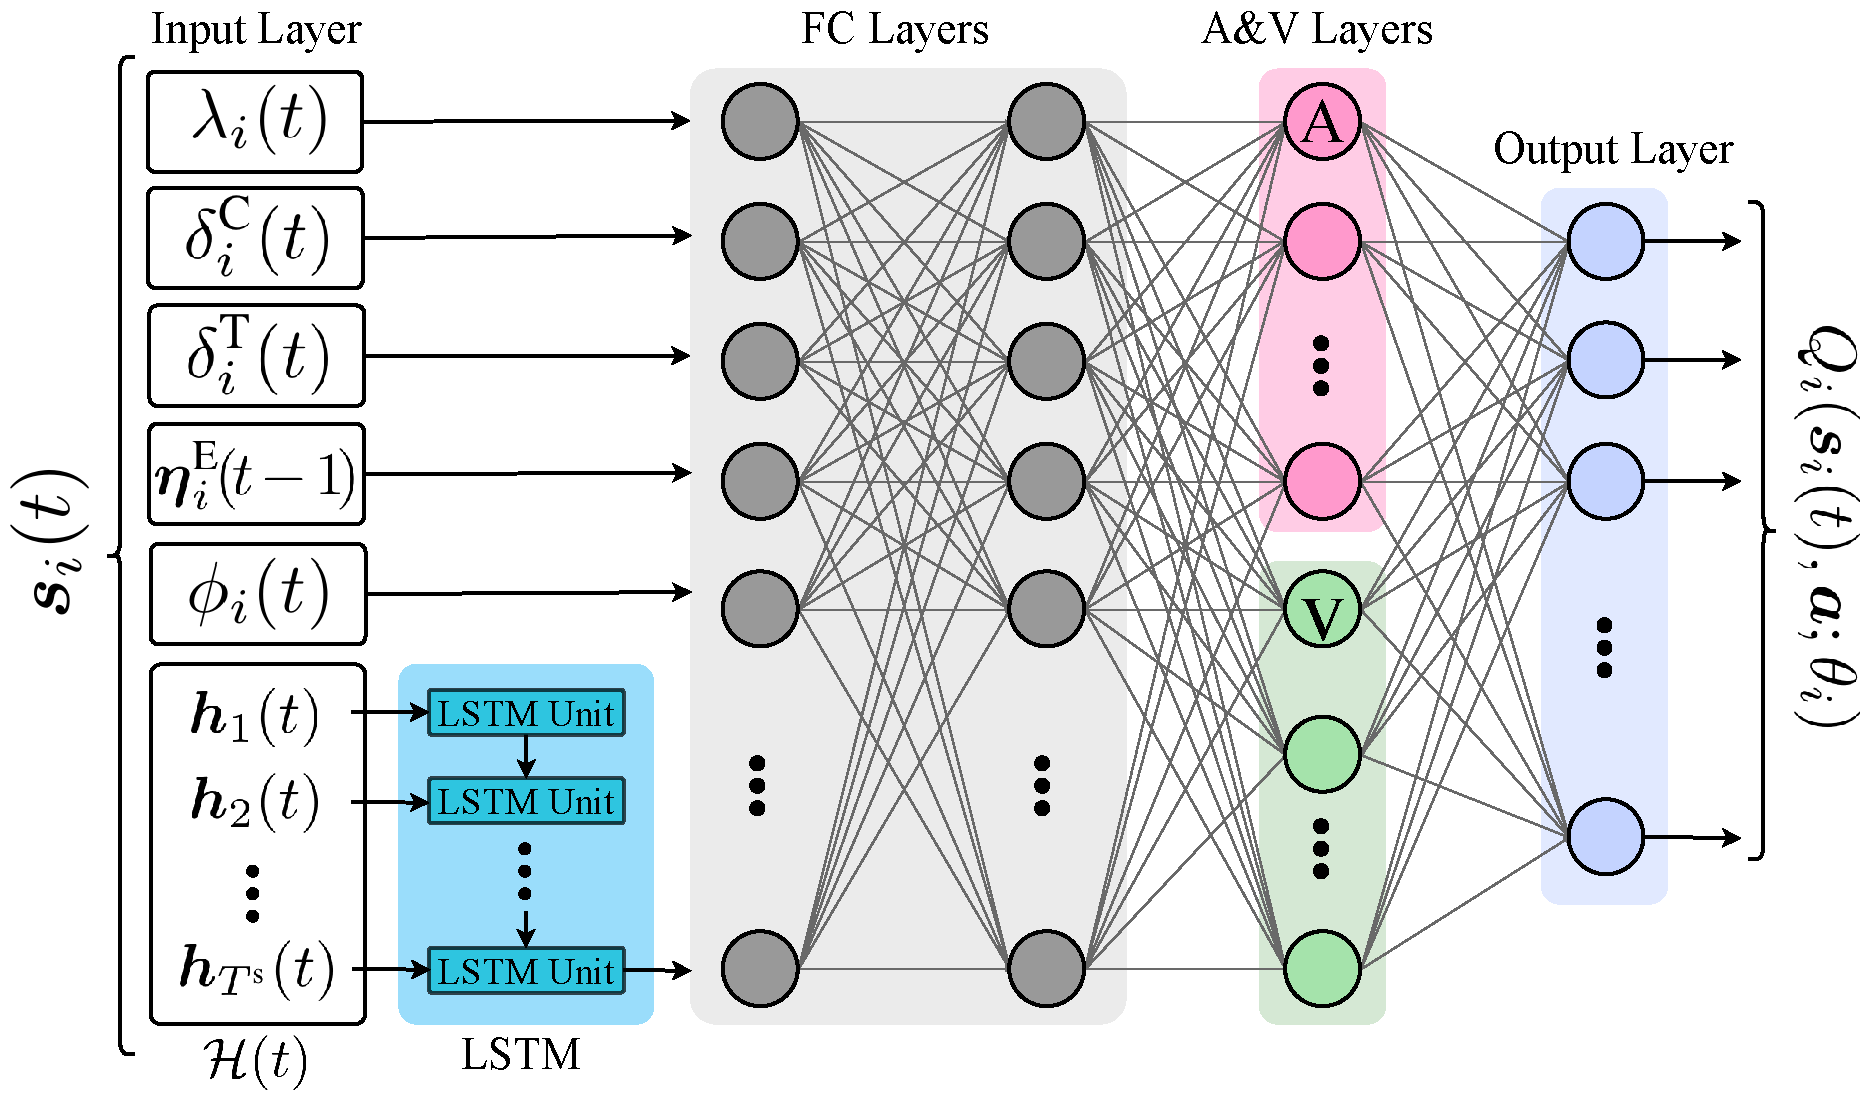
\includegraphics[width=0.85\linewidth]{DQN}
	\vspace*{-5mm}
	%\caption{An illustration MD $i \in \mathcal{I}$ and EN $j \in \mathcal{J}$ in the MEC system.}
	\vspace*{-3mm}
	\label{fig1}
\end{figure}
	
	\vspace{6mm}
	
	\begin{itemize}[]
	
	\item  \hspace{0mm}  \textcolor{teal}{LSTM}: ENs Load Level Prediction
	
	\item  \hspace{0mm}  \textcolor{teal}{FC}: State-Action Q-Value Mapping
	
	
	\item \hspace{0mm}  \textcolor{teal}{A\&V}: Dueling-DQN Approach for Q-Value Estimation
	
	
	
	
\end{itemize}

	
\end{frame}


\begin{frame}
	\frametitle{QOCO Algorithm}
	
	\textbf{Offloading Decision Algorithm at MD}
	

	\vspace{6mm}
	
	\begin{itemize}[]
		
		\item Offloading Decision Algorithm at MD
		
		
		\item Training Process Algorithm at EN
		
		
	\end{itemize}
	
	
\end{frame}

\begin{frame}
	\frametitle{QOCO Algorithm}
	
	\textbf{Training Process Algorithm at EN}
	
	
	\vspace{6mm}
	
	\begin{itemize}[]
		
		\item Offloading Decision Algorithm at MD
		
		
		\item Training Process Algorithm at EN
		
		
	\end{itemize}
	
	
\end{frame}